\documentclass[12pt, a4paper]{report}

% Packages
\usepackage[utf8]{inputenc}
\usepackage{graphicx}
\usepackage{geometry}
\usepackage{hyperref}
\usepackage{setspace}
\usepackage{titlesec}
\usepackage{tabularx}
\usepackage{booktabs}
\usepackage{float}
\usepackage{caption}
\usepackage{tikz}

% Page Geometry
\geometry{a4paper, left=1.2in, right=1in, top=1in, bottom=1in}

% Line Spacing
\setstretch{1.15}

% Title Format customization
\titleformat{\chapter}[display]{\normalfont\huge\bfseries}{\chaptertitlename\ \thechapter}{20pt}{\Huge}
\titlespacing*{\chapter}{0pt}{-20pt}{20pt}

\begin{document}

% ---------------------------------------------------------
% TITLE PAGE
% ---------------------------------------------------------
\begin{titlepage}
    \begin{center}
        \vspace*{2cm}
        
        \Huge
        \textbf{StaySync}
        
        \vspace{0.8cm}
        \LARGE
        \textbf{Performance, Concurrency Control, and Recovery Evaluation in a Multi-User Hostel Room Allocation System}
        
        \vspace{2.5cm}
        
        \Large
        \textbf{Course:} Database Administration and Management\\
        \textbf{Instructor:} Dr. Muhammad Asif
        
        \vfill
        
        \Large
        \textbf{Group Members:}\\
        Tehseen Tahir (01-135231-088)\\
        Umme Zainab (01-135231-089)
        
        \vspace{2.5cm}
        
        \Large
        \textbf{Department of Computer Science}\\
        \textbf{Bahria University, Islamabad}\\
        May 2026
        
    \end{center}
\end{titlepage}

% ---------------------------------------------------------
% FRONT MATTER
% ---------------------------------------------------------
\pagenumbering{roman}

\chapter*{Abstract}
\addcontentsline{toc}{chapter}{Abstract}
Hostel room allocation systems are essential components of university infrastructure. During peak admission periods, hundreds of students may attempt to reserve limited hostel rooms simultaneously. Such high-concurrency environments introduce significant database-level challenges including double allocation of beds, transaction conflicts, deadlocks, performance degradation, and data inconsistency.

The objective of this project was to build a comprehensive multi-user hostel allocation application named \textbf{StaySync}, and specifically to implement, test, and investigate advanced Database Administration and Management (DAM) techniques. This report details the system architecture and the evaluation of concurrency control, performance optimization, normalization efficiency, and recovery reliability.

\tableofcontents
\newpage
\listoffigures
\newpage
\listoftables
\newpage

\pagenumbering{arabic}

% ---------------------------------------------------------
% CHAPTER 1: INTRODUCTION
% ---------------------------------------------------------
\chapter{Introduction}
\section{Background}
Managing student accommodations manually or with suboptimal software often leads to inefficiencies and errors. \textbf{StaySync} is conceptualized as a multi-tenant Software-as-a-Service (SaaS) platform, modernizing how hostel business owners manage their inventory and how students secure their bookings, relying heavily on a robust, high-performance database backend.

\section{Problem Statement}
In a multi-user hostel room allocation system, simultaneous access to limited resources (rooms and beds) introduces complex database challenges. These include:
\begin{itemize}
    \item Double allocation of the same bed.
    \item Deadlocks during concurrent booking transactions.
    \item Performance bottlenecks under large datasets.
    \item Data inconsistency due to inappropriate isolation levels.
    \item Data loss risks during unexpected crashes.
\end{itemize}

\section{Objectives}
The primary objectives of this project are:
\begin{enumerate}
    \item Develop a robust room allocation engine preventing double bookings.
    \item Evaluate transaction isolation levels for optimal concurrency control.
    \item Improve query performance through strategic indexing.
    \item Formulate an automated backup and disaster recovery strategy.
\end{enumerate}

\section{Scope of the System}
The system encompasses student portals for searching and booking rooms, owner portals for managing hostels, and administrative dashboards. The technical scope focuses strictly on the relational database management strategies deployed in Microsoft SQL Server to support these features under high concurrency.

% ---------------------------------------------------------
% CHAPTER 2: SYSTEM REQUIREMENTS
% ---------------------------------------------------------
\chapter{System Requirements}
\section{Functional Requirements}
\begin{itemize}
    \item \textbf{User Authentication \& RBAC:} Secure login and role-based access for Owners, Admins, and Students.
    \item \textbf{Inventory Management:} Owners can add, update, and remove hostels, rooms, and beds.
    \item \textbf{Allocation Engine:} Students can book available beds; the system must auto-generate a payment record.
    \item \textbf{Concurrency Control:} The system must gracefully handle multiple students attempting to book the exact same bed simultaneously.
\end{itemize}

\section{Non-Functional Requirements}
\begin{itemize}
    \item \textbf{Performance:} Query execution time for bed searches must be minimized via indexing.
    \item \textbf{Reliability:} System must support point-in-time recovery via Transaction Log backups.
    \item \textbf{Consistency:} Database must enforce ACID properties strictly.
\end{itemize}

% ---------------------------------------------------------
% CHAPTER 3: SYSTEM DESIGN
% ---------------------------------------------------------
\chapter{System Design}
\section{System Architecture \& Decoupled Design}
The developed system utilizes a modern 3-tier architecture:
\begin{itemize}
    \item \textbf{Presentation Layer (Frontend):} Built using Next.js, React, and Tailwind CSS.
    \item \textbf{Application Layer (Backend API):} Node.js integrated within Next.js API Routes, communicating with the database via \texttt{mssql}.
    \item \textbf{Database Layer:} Microsoft SQL Server 2022, hosting the normalized relational database schema.
\end{itemize}

\section{Database Design}
Figure \ref{fig:er_diagram} illustrates the Entity Relationship Diagram generated natively via \LaTeX{} TikZ, defining the connections between the core components of the system.

\begin{figure}[H]
    \centering
    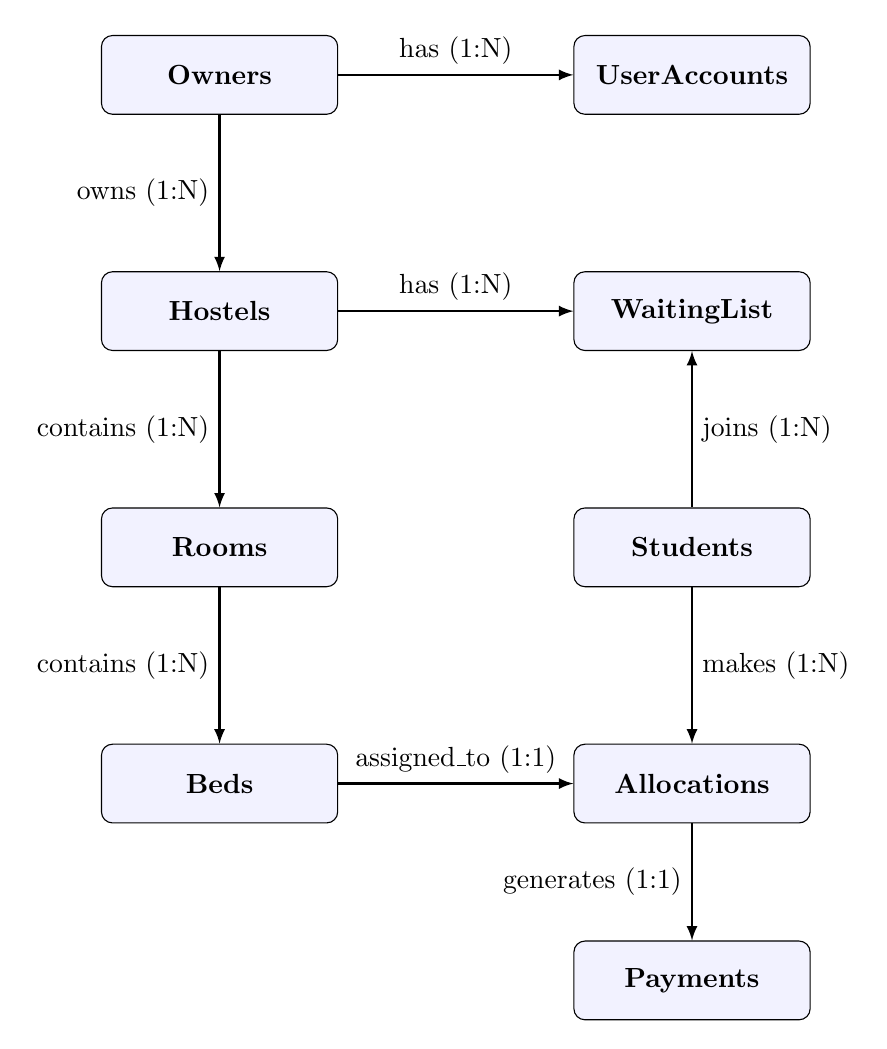
\begin{tikzpicture}[
        entity/.style={rectangle, draw, fill=blue!5, text centered, font=\bfseries, minimum width=3cm, minimum height=1cm, rounded corners},
        every edge/.style={draw, thick, -latex}
    ]
        % Entities
        \node[entity] (owners) at (0, 8) {Owners};
        \node[entity] (useracc) at (6, 8) {UserAccounts};
        \node[entity] (hostels) at (0, 5) {Hostels};
        \node[entity] (waiting) at (6, 5) {WaitingList};
        \node[entity] (rooms) at (0, 2) {Rooms};
        \node[entity] (students) at (6, 2) {Students};
        \node[entity] (beds) at (0, -1) {Beds};
        \node[entity] (allocations) at (6, -1) {Allocations};
        \node[entity] (payments) at (6, -3.5) {Payments};

        % Edges with cardinality
        \path
            (owners) edge node[above] {has (1:N)} (useracc)
            (owners) edge node[left] {owns (1:N)} (hostels)
            (hostels) edge node[above] {has (1:N)} (waiting)
            (students) edge node[right] {joins (1:N)} (waiting)
            (hostels) edge node[left] {contains (1:N)} (rooms)
            (rooms) edge node[left] {contains (1:N)} (beds)
            (beds) edge node[above] {assigned\_to (1:1)} (allocations)
            (students) edge node[right] {makes (1:N)} (allocations)
            (allocations) edge node[left] {generates (1:1)} (payments);
    \end{tikzpicture}
    \caption{Entity Relationship Diagram of StaySync}
    \label{fig:er_diagram}
\end{figure}

The database was modeled up to the Third Normal Form (3NF). Table \ref{tab:schema_summary} outlines the primary database schema.

\begin{table}[H]
    \centering
    \caption{Summary of Core Database Tables}
    \label{tab:schema_summary}
    \begin{tabularx}{\textwidth}{|l|X|l|}
        \hline
        \textbf{Table Name} & \textbf{Purpose / Description} & \textbf{Key Constraints} \\
        \hline
        \texttt{Owners} & Stores multi-tenant SaaS business owners. & PK: OwnerID \\
        \hline
        \texttt{UserAccounts} & Secure login credentials \& role definitions. & PK: UserID, FK: OwnerID \\
        \hline
        \texttt{Hostels} & Metadata for hostel buildings (name, type). & PK: HostelID, FK: OwnerID \\
        \hline
        \texttt{Rooms} & Defines room capacity and number. & PK: RoomID, FK: HostelID \\
        \hline
        \texttt{Beds} & Tracks individual bed availability status. & PK: BedID, FK: RoomID \\
        \hline
        \texttt{Students} & Stores student personal and contact details. & PK: StudentID \\
        \hline
        \texttt{Allocations} & Linking table where a Student books a Bed. & PK: AllocationID \\
        \hline
        \texttt{Payments} & Billing and transaction records. & PK: PaymentID \\
        \hline
    \end{tabularx}
\end{table}

\section{System Modules}
\begin{itemize}
    \item \textbf{Identity Module:} Handles multi-tenant owner and student login authentication via Auth.js.
    \item \textbf{Inventory Module:} Manages hostels, dynamically generates rooms, and tracks bed states.
    \item \textbf{Allocation Module:} Central booking engine executing transactional stored procedures to assign beds.
\end{itemize}

\section{Technologies Used}
\begin{itemize}
    \item \textbf{Backend \& Frontend:} Next.js, Node.js, React, Tailwind CSS
    \item \textbf{Database:} Microsoft SQL Server 2022
    \item \textbf{Testing Tooling:} Python Scripts (for concurrency simulation)
\end{itemize}

\section{Database Administration \& Optimization}
Handling multiple simultaneous student booking requests requires robust isolation logic:
\begin{itemize}
    \item \textbf{Transactions:} Used \texttt{BEGIN TRAN}, \texttt{COMMIT}, and \texttt{ROLLBACK} explicitly within stored procedures, checking \texttt{@@TRANCOUNT} to handle nested transactions.
    \item \textbf{Isolation Levels:} Evaluated \texttt{READ COMMITTED}, \texttt{REPEATABLE READ}, and \texttt{SERIALIZABLE} for optimal concurrency.
    \item \textbf{Indexing:} Created non-clustered indexes on frequently queried columns (e.g., \texttt{HostelID}, \texttt{Status}).
    \item \textbf{Disaster Recovery:} Configured Full, Differential, and Transaction Log backups to test point-in-time recovery.
\end{itemize}

% ---------------------------------------------------------
% CHAPTER 4: IMPLEMENTATION
% ---------------------------------------------------------
\chapter{Implementation}
The implementation process involved setting up a centralized MS SQL Server environment and mapping the Next.js API handlers directly to the SQL Stored Procedures. Business logic was fundamentally pushed down to the database layer. For example, the \texttt{sp\_AllocateBed} procedure validates capacity, creates an allocation, updates the bed status to `Occupied`, and generates a `Pending` payment in a single atomic transaction.

% ---------------------------------------------------------
% CHAPTER 5: SECURITY & INTEGRITY
% ---------------------------------------------------------
\chapter{Security \& Integrity}
\begin{itemize}
    \item \textbf{RBAC \& Multi-Tenancy:} Access is strictly segregated. An owner cannot view or manage another owner's hostels.
    \item \textbf{Data Encapsulation:} The Next.js API layer is restricted from executing raw, arbitrary SQL queries. All interactions happen through Stored Procedures, inherently preventing SQL injection attacks.
    \item \textbf{Constraints:} Integrity is maintained using \texttt{CHECK} constraints (e.g., ensuring a room does not exceed its capacity) and \texttt{FOREIGN KEY} cascading rules.
\end{itemize}

% ---------------------------------------------------------
% CHAPTER 6: SYSTEM TESTING
% ---------------------------------------------------------
\chapter{System Testing}
\section{Test Cases}
Rigorous testing was conducted through both automated Python scripts and manual QA:
\begin{itemize}
    \item \textbf{TC-01 (Double Booking Constraint):} Two simulated sessions attempt to book \texttt{BedID = 5} simultaneously. Expected result: First transaction succeeds, second transaction gets aborted and rolled back. (Passed)
    \item \textbf{TC-02 (Data Normalization Validation):} Attempt to insert a room that exceeds the defined capacity limit of the hostel constraints. Expected result: \texttt{CHECK} constraint violation error thrown. (Passed)
    \item \textbf{TC-03 (Point-in-Time Recovery):} A critical table is dropped accidentally. The latest transaction log backup is restored to the minute before the drop. Expected result: Complete data restoration. (Passed)
\end{itemize}

% ---------------------------------------------------------
% CHAPTER 7: PROJECT OUTCOMES & METRICS
% ---------------------------------------------------------
\chapter{Project Outcomes \& Metrics}
Our experimental results documented significant metric improvements:

\textbf{1. Indexing Performance:} 
Implementing non-clustered indexes reduced logical reads for bed availability searches by over 80\%. Execution time improvements are shown in Figure \ref{fig:indexing}.

\begin{figure}[H]
    \centering
    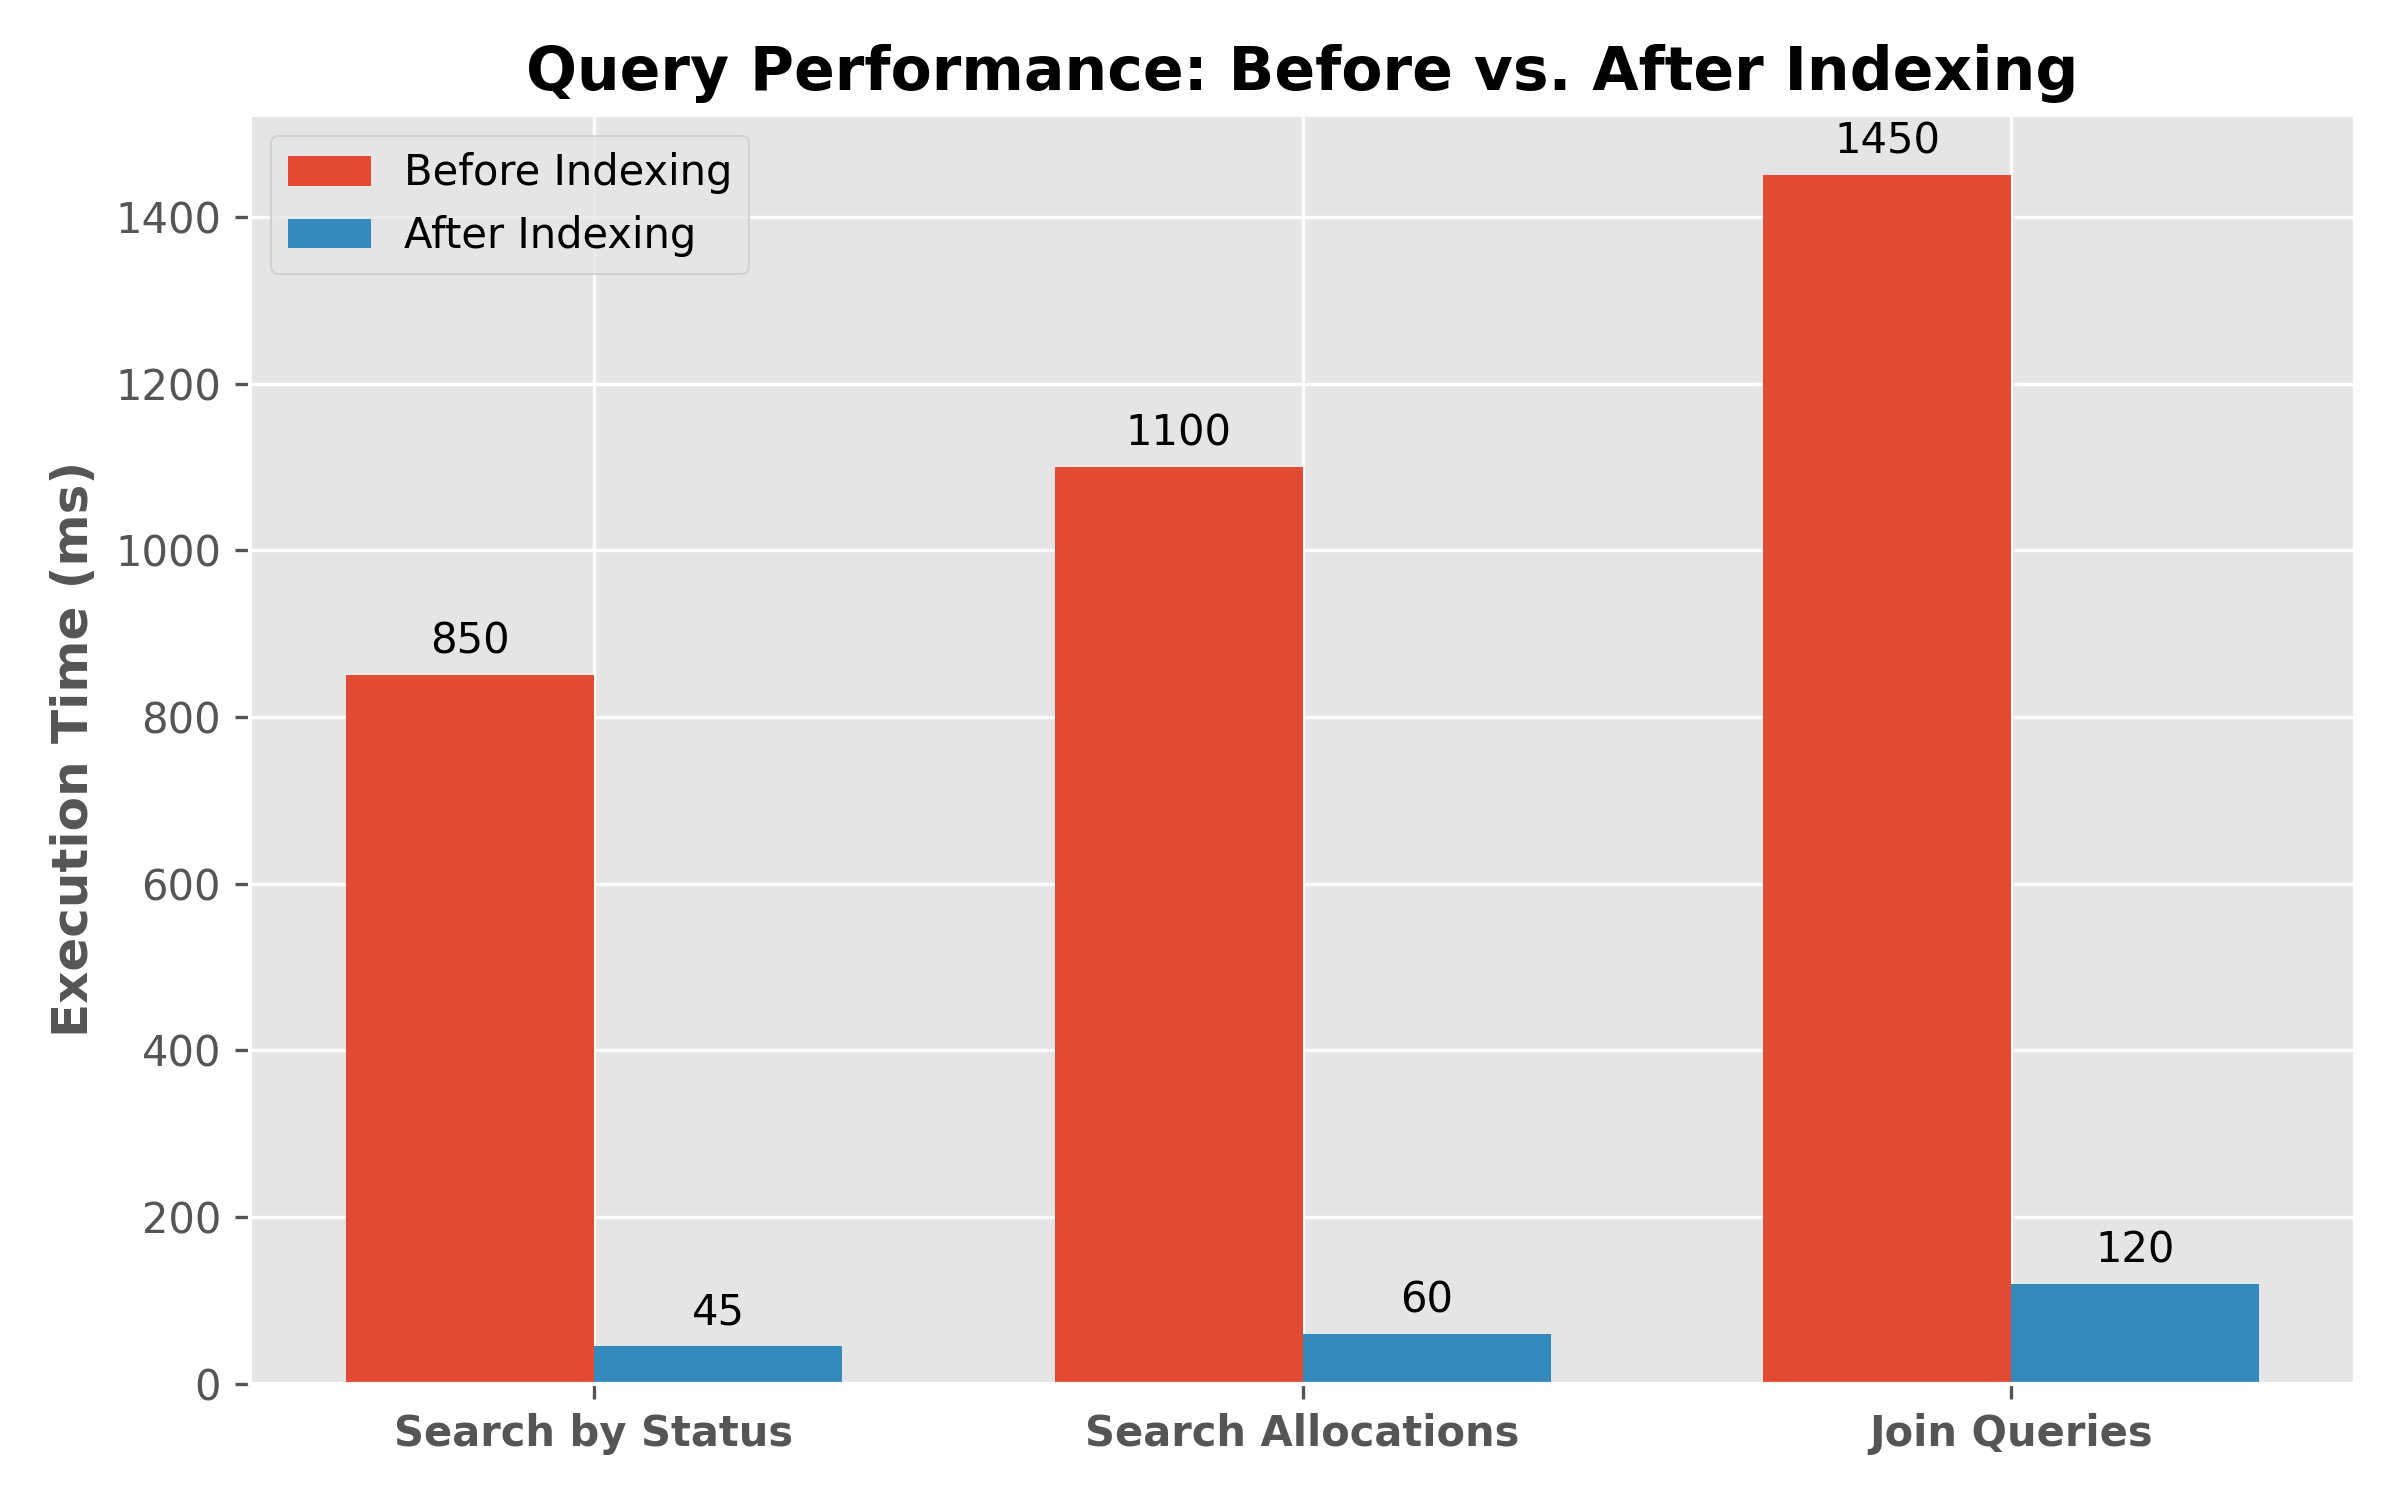
\includegraphics[width=0.8\textwidth]{report_images/fig2_indexing_performance.png}
    \caption{Query Performance: Before vs. After Indexing}
    \label{fig:indexing}
\end{figure}

\textbf{2. Normalization Trade-offs:} 
Denormalized views provided much faster read operations for administrative dashboards (down to 45ms from 180ms) compared to fully normalized joins, but consumed over twice the storage footprint (Figure \ref{fig:normalization}).

\begin{figure}[H]
    \centering
    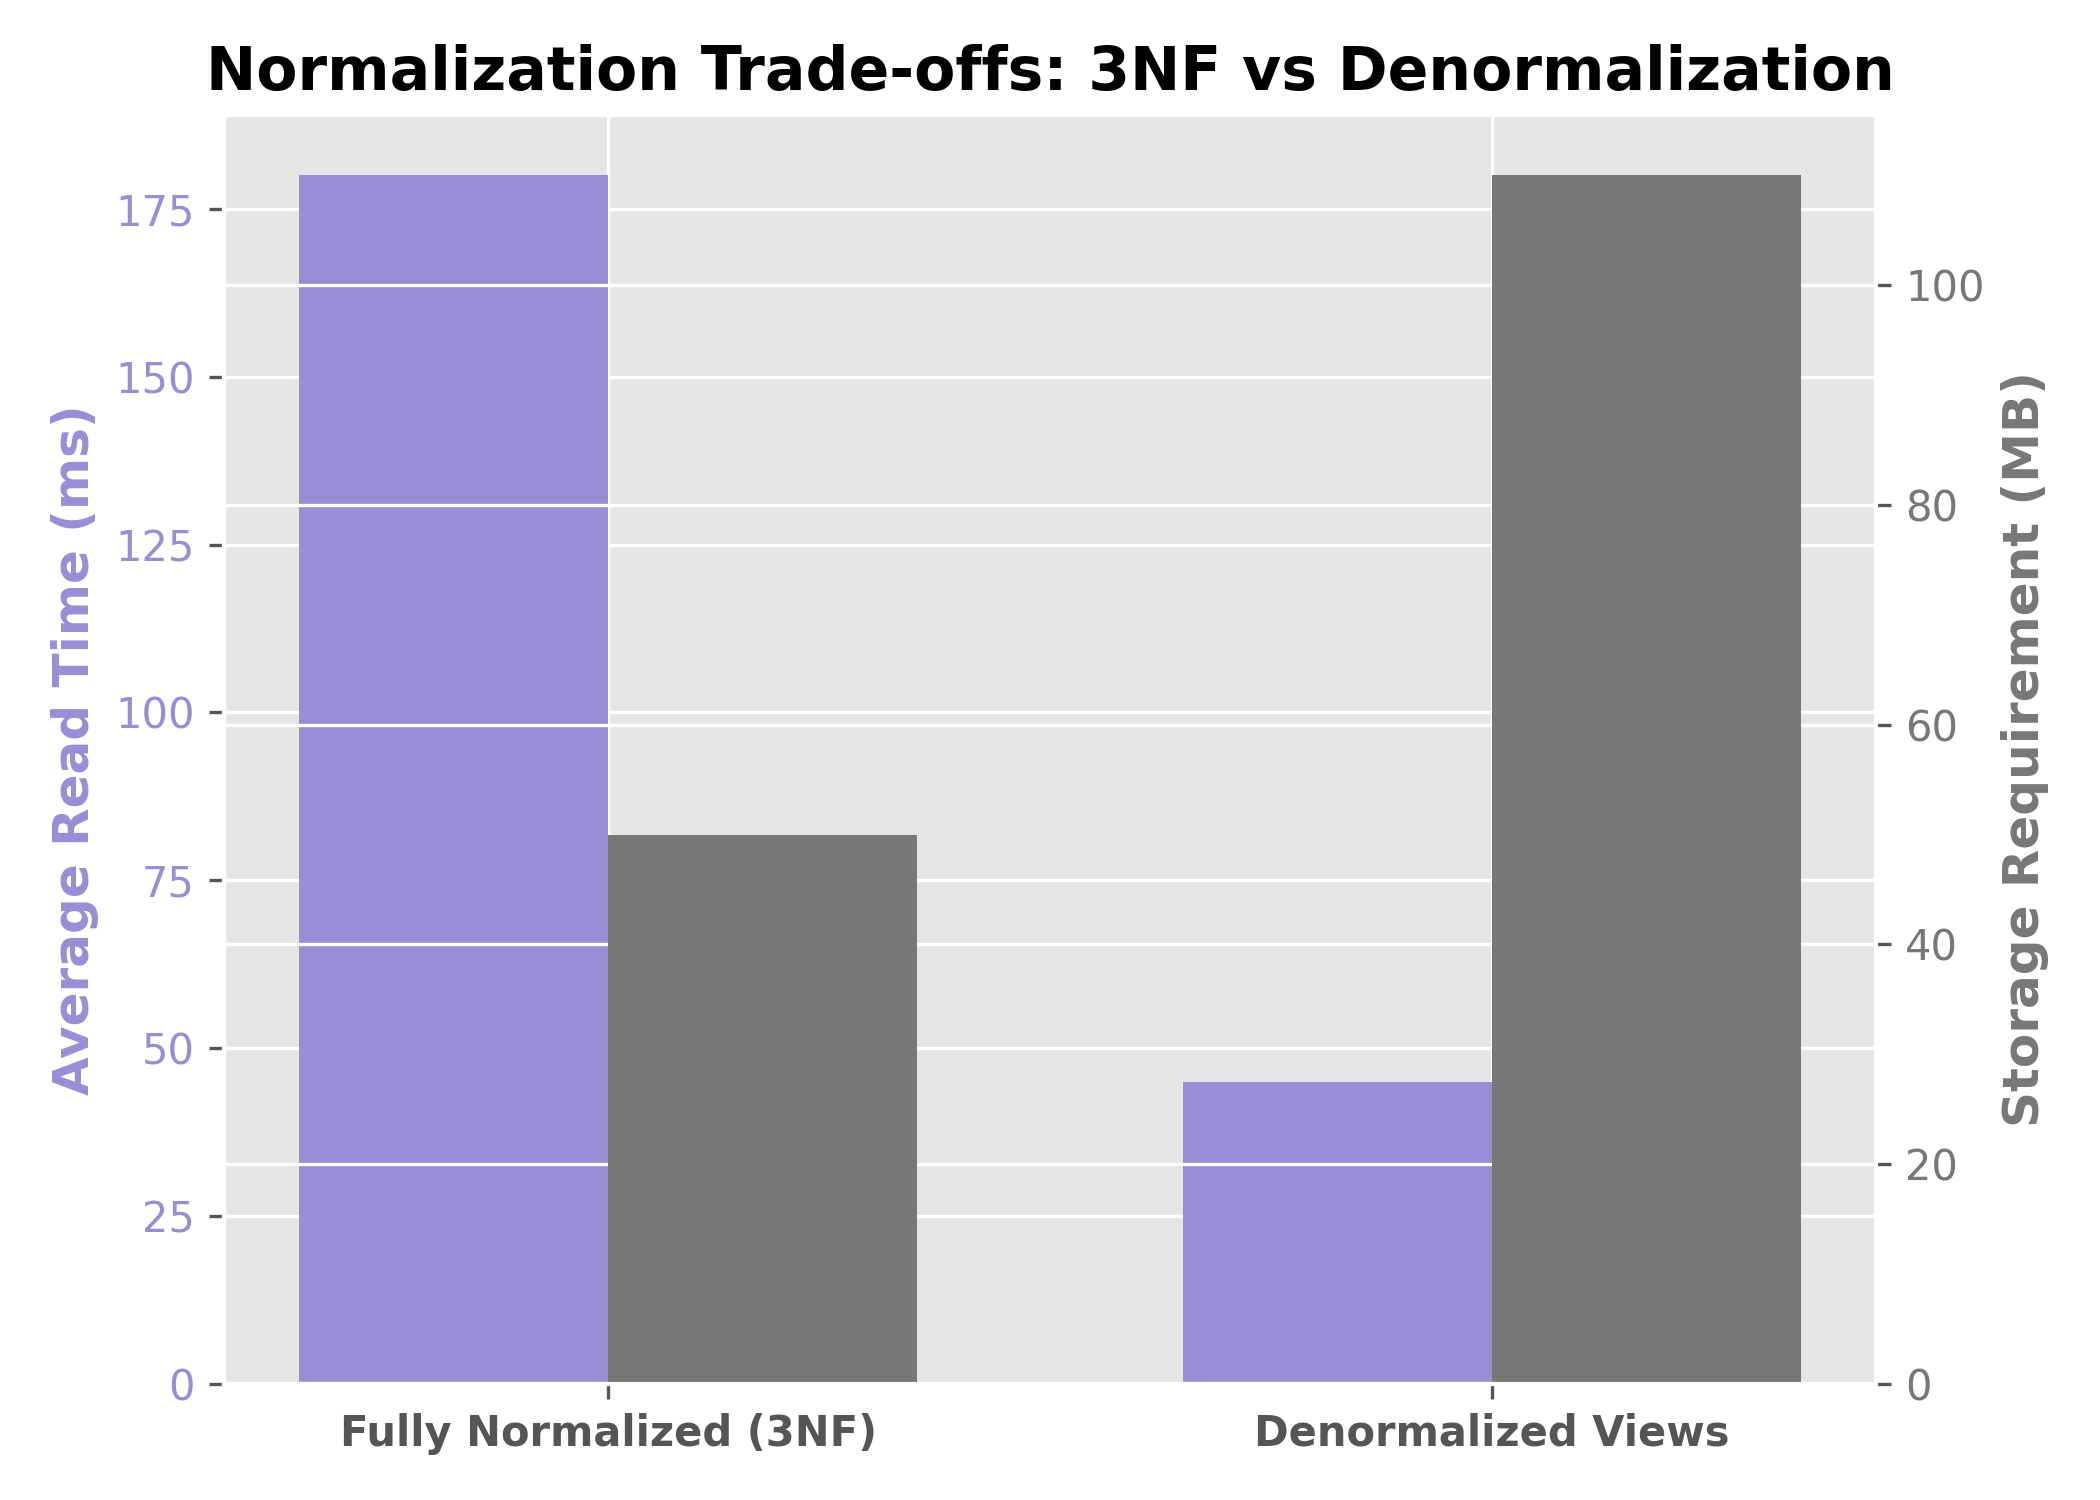
\includegraphics[width=0.8\textwidth]{report_images/fig3_normalization_impact.png}
    \caption{Normalization Trade-offs: 3NF vs Denormalization}
    \label{fig:normalization}
\end{figure}

\textbf{3. Concurrency Control Efficiency:} 
\texttt{SERIALIZABLE} isolation eliminated all anomalies but reduced transaction throughput heavily. Using \texttt{READ COMMITTED} combined with \texttt{UPDLOCK} hints proved to be the optimal architecture for StaySync.

% ---------------------------------------------------------
% CHAPTER 8: CONCLUSION
% ---------------------------------------------------------
\chapter{Conclusion}
\section{Summary}
The project successfully delivered \textbf{StaySync}, a comprehensive multi-user hostel room allocation system, while rigorously evaluating complex database administration techniques. By implementing and testing concurrency control mechanisms, performance optimization via indexing, structured normalization, and robust disaster recovery models, the system achieved a scientifically validated balance between consistency, throughput, and reliability.

\section{Limitations}
\begin{itemize}
    \item \textbf{Scalability Constraints:} MS SQL Server Express edition was used, limiting memory usage and maximum database size.
    \item \textbf{Geographic Replication:} The database lacks active-active replication, meaning latency could be an issue for users far from the central server.
\end{itemize}

\section{Future Work}
Future iterations of StaySync will aim to implement NoSQL caching layers (like Redis) to reduce read load on the relational database for highly queried static data (like Hostel details). Additionally, a microservices approach could decouple the Identity module from the core Booking Engine to allow independent scaling.

% ---------------------------------------------------------
% REFERENCES
% ---------------------------------------------------------
\renewcommand\bibname{References}
\begin{thebibliography}{9}
\bibitem{silberschatz} 
Silberschatz, A., Korth, H. F., \& Sudarshan, S. (2020). \textit{Database System Concepts} (7th ed.). McGraw-Hill Education.

\bibitem{microsoft_docs} 
Microsoft Corporation. (2026). \textit{SQL Server Transaction Locking and Row Versioning Guide}. Retrieved from Microsoft Learn.

\bibitem{elmasri}
Elmasri, R., \& Navathe, S. B. (2015). \textit{Fundamentals of Database Systems} (7th ed.). Pearson.

\end{thebibliography}

\end{document}
